\documentclass[10pt,a4paper,landscape]{article}
\usepackage{multicol}
\usepackage{calc}
\usepackage{ifthen}
\usepackage[landscape]{geometry}
\usepackage{amsmath,amsthm,amsfonts,amssymb}
\usepackage{color,graphicx}
\usepackage{hyperref}
\usepackage{listings}
\usepackage{underscore}
\usepackage{todonotes}

% Cheatsheet style
% Cheatsheet style

% This sets page margins to .5 inch if using letter paper, and to 1cm
% if using A4 paper. (This probably isn't strictly necessary.)
% If using another size paper, use default 1cm margins.
\ifthenelse{\lengthtest{\paperwidth = 11in}}
  % Then
  { \geometry{top=.5in,left=.5in,right=.5in,bottom=.5in} }
  % Else
  { \ifthenelse{\lengthtest{\paperwidth = 297mm}}
    {\geometry{top=1cm,left=1cm,right=1cm,bottom=1cm} }
    {\geometry{top=1cm,left=1cm,right=1cm,bottom=1cm} }
  }

% Turn off header and footer
\pagestyle{empty}

% Redefine section commands to use less space
\makeatletter
\renewcommand{\section}{\@startsection{section}{1}{0mm}%
                                {-1ex plus -.5ex minus -.2ex}%
                                {0.5ex plus .2ex}%x
                                {\color{darkred}\normalfont\large\bfseries}}
\renewcommand{\subsection}{\@startsection{subsection}{2}{0mm}%
                                {-1explus -.5ex minus -.2ex}%
                                {0.5ex plus .2ex}%
                                {\color{darkdarkred}\normalfont\normalsize\bfseries}}
\renewcommand{\subsubsection}{\@startsection{subsubsection}{3}{0mm}%
                                {-1ex plus -.5ex minus -.2ex}%
                                {1ex plus .2ex}%
                                {\normalfont\small\bfseries}}
\makeatother

% Define BibTeX command
\def\BibTeX{{\rm B\kern-.05em{\sc i\kern-.025em b}\kern-.08em
    T\kern-.1667em\lower.7ex\hbox{E}\kern-.125emX}}

% Don't print section numbers
\setcounter{secnumdepth}{0}

\setlength{\parindent}{0pt}
\setlength{\parskip}{0pt plus 0.5ex}

% Setting colors
\definecolor{lightgray}{rgb}{0.7,0.7,0.7}
\definecolor{lightergray}{rgb}{0.9,0.9,0.9}
\definecolor{darkblue}{rgb}{0.4,0.4,1}
\definecolor{darkred}{rgb}{0.9,0.2,0.2}
\definecolor{darkdarkred}{rgb}{0.6,0.0,0.0}
\definecolor{lightred}{rgb}{1,0.6,0.6}
\definecolor{lightgreen}{rgb}{0.6,1,0.6}
\definecolor{lightblue}{rgb}{0.6,0.8,1}
\definecolor{darkgreen}{rgb}{0.4,1,0.4}

% Set code listing style
\lstset {
    backgroundcolor=\color{lightgray},
    basicstyle=\ttfamily\scriptsize,
    breaklines=true,
}

\lstdefinestyle{bb}{
    backgroundcolor=\color{lightergray},
    frame=L,
    xleftmargin=\parindent,
}

% Set hyperlink style
\hypersetup{hidelinks}

% Enable figures
\newenvironment{colfig}
  {\par\medskip\noindent\minipage{\linewidth}}
  {\endminipage\par\medskip}

% Enable arg min/max math operators
\DeclareMathOperator*{\argmin}{arg\,min}
\DeclareMathOperator*{\argmax}{arg\,max}


% Shorthands
\providecommand{\bf}[1]{\ensuremath{\bf{#1}}}
\newcommand{\E}{\mathrm{E}}
\newcommand{\Var}{\mathrm{Var}}
\newcommand{\Cov}{\mathrm{Cov}}

\pdfinfo{
  /Title (Machine Learning Cheat Sheet)
  /Creator (TeX)
  /Producer (pdfTeX 1.40.0)
  /Author (Dennis Meier)
  /Subject (Machine Learning cheatsheet)
  /Keywords (machinelearning, ml, bayes, regression, classification)
}

% -----------------------------------------------------------------------

\begin{document}
\title{Machine Learning Cheat Sheet}

\raggedright
\footnotesize
\sffamily
\begin{multicols*}{4}

% multicol parameters
% These lengths are set only within the two main columns
%\setlength{\columnseprule}{0.25pt}
\setlength{\premulticols}{1pt}
\setlength{\postmulticols}{1pt}
\setlength{\multicolsep}{1pt}
\setlength{\columnsep}{2pt}

\begin{center}
\Large{\underline{Machine Learning Cheat Sheet}}
\end{center}

% ----------
\section{General}
\subsection{Dataset and Definitions}
$\mathcal{D}$ is a set of training examples, the n-th Training Example ($n = 1,2, ..., N$), of this set is: $\bf{x}_n = \begin{bmatrix} x_{n1} \quad x_{n2} \quad ... \quad x_{nD} \end{bmatrix} $

We write all N training examples in a matrix: $\bf{X} = \begin{bmatrix} \bf{x}_1 ; \quad \bf{x}_2 ; \quad ... ; \quad \bf{x}_N \end{bmatrix}$

In supervised learning, you are also given a set of observations corresponding to the training examples:  $\bf{y} = \begin{bmatrix} y_1 \quad y_2 \quad ... \quad y_{N} \end{bmatrix}^T$

We assume a \emph{true} model behind the data, the observations are noisy versions of this ground truth: $y = y_{true} + \epsilon$.

The final goal is to predict a $\hat{y}$ given any $\bf{x}$.

\subsection{Distributions}
Multivariate gaussian distribution: $\mathcal{N}(\bf{X} | \bf{\mu} , \bf{\Sigma})$ \\
$\implies p(\bf{X} = \bf{x}) = (2 \pi)^{-d/2} |\bf{\Sigma|}^{-1/2} \exp{[- \frac{1}{2} (\bf{x} - \bf{\mu})^T \bf{\Sigma}^{-1} (\bf{x} - \bf{\mu})]}$

Gaussian distribution: $\mathcal{N}(X| \mu, \sigma^2)$ \\
$\implies p(X = x) = \frac{1}{\sqrt{2 \pi \sigma^2}} \exp{(- \frac{1}{2} ( \frac{x - \mu}{\sigma} )^2)}$

Poisson distribution: $\mathcal{P}(X| \lambda)$ \\
$\implies p(X = k) = \frac{\lambda ^ k}{k!} \exp{(- \lambda)}$

% ----------
\section{Optimization methods}

\subsection{Grid Search}
Simply try values for all parameters at regular intervals.
Complexity: $\mathcal{O}(M^D N D)$, where $M$ is the number of values tried in each dimension.

\subsection{Gradient Descent}
Update rule: $\boldsymbol\beta^{(k+1)} = \boldsymbol\beta^{(k)} - \alpha \frac{\partial \mathcal{L}(\boldsymbol\beta^{(k)})}{\partial \boldsymbol\beta}$

Complexity: $\mathcal{O}(I N D)$ where $I$ is the number of iterations we take.

$\alpha$ is a parameter that needs to be chosen carefully.

The gradient for MSE comes out as:
$\frac{\partial \mathcal{L}}{\partial \boldsymbol\beta} = - \frac{1}{N} \tilde{X}^T ( \boldsymbol y - \tilde{X} \boldsymbol\beta )$

\subsection{Newton's method}
It uses second order derivatives information to converge faster (we approximate the objective function by a quadratic function rather than a line).

General rule: $\boldsymbol\beta^{(k+1)} = \boldsymbol\beta^{(k)} - \alpha \bf{H_k^{-1}} \frac{\partial \mathcal{L}(\boldsymbol\beta^{(k)})}{\partial \boldsymbol\beta}$\\
where $\bf{H_k}$ is the $D \times D$ Hessian at step $k$: $\bf{H_k} = \frac{\partial^2 \mathcal{L}(\boldsymbol\beta^{(k)})}{\partial \boldsymbol\beta^2}$

Newton's method is equivalent to solving many least-squares problems.

Complexity: $\mathcal{O}(I N D^2 + I D^3)$, with the $D^3$ cost coming from the inversion of $\bf{H_k}$.

% ----------
\section{Regression}
Simple linear regression: $y_n \approx \beta_0 + \beta_1 x_{n1}$

Multiple linear regression: $y_n \approx f(\bf{x}_n) := \beta_0 + \beta_1 x_{n1} + \beta_2 x_{n2} + ... + \beta_D x_{nD}$

\subsection{Linear basis function model}
$y_n = \beta_0 + \sum_{i=1}^{M} \beta_i \phi_i(\bf{x_n}) =  \bf{\tilde\phi^T}(\bf{x}^T_n) \boldsymbol\beta$.
The optimal $\beta$ is given by $\beta = ( \tilde{\Phi}^T \tilde{\Phi})^{-1} \tilde{\Phi}^T y$ where $\tilde{\Phi}$ is a matrix with N rows and the n-th row is $[1, \phi_1(x_n)^T,  ...,  \phi_M(x_n)^T]$.

Ridge regression: $\beta_{ridge} = ( \tilde{\boldsymbol \Phi}^T \tilde{\boldsymbol\Phi} + \lambda \boldsymbol I)^{-1} \tilde{\boldsymbol\Phi}^T \boldsymbol y$

\subsection{Cost functions}
\begin{colfig}
\centering
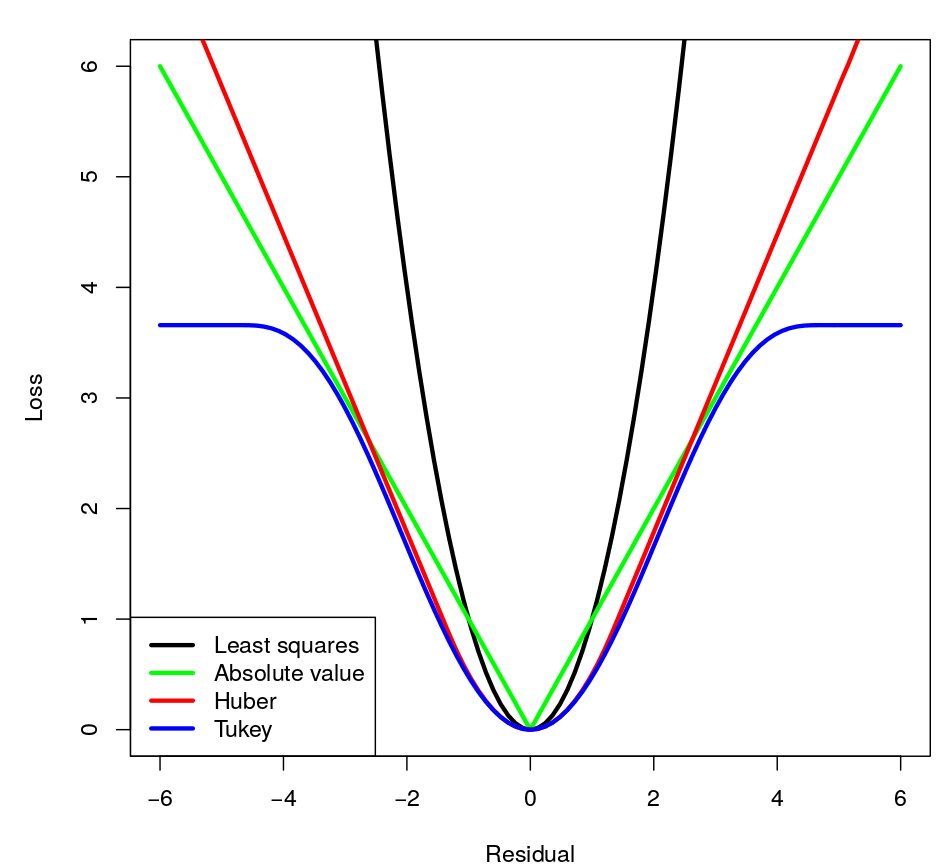
\includegraphics[width=\linewidth]{images/error-functions.png}
\end{colfig}

Cost function / Loss: $\mathcal{L}(\boldsymbol\beta) = \mathcal{L}(\mathcal{D},\boldsymbol\beta)$

Mean square error (MSE): $\frac{1}{2N} \sum_{n=1}^{N}\left[y_n-f(\bf{x}_i) \right]^2$

MSE matrix formulation: $\frac{1}{2N} (\bf{y - X \beta})^T (\bf{y - X \beta})$

Mean absolute error (MAE): $\frac{1}{2N} \sum_{n=1}^{N}\left | y_n-f(\bf{x}_i) \right |$

Huber loss: $\mathcal{L}_\delta (a) = \begin{cases}
\frac{1}{2}{a^2}                   & \text{for } |a| \le \delta, \\
\delta (|a| - \frac{1}{2}\delta ), & \text{otherwise.}
\end{cases}$

Root mean square error (RMSE): $\sqrt{2 * \text{MSE}}$

Epsilon insensitive (``hinge loss'', used for SVM):
$\mathcal{L}_{\epsilon}(y, \hat{y}) = \begin{cases}
0                   & \text{if } |y - \hat y| \le \epsilon, \\
|y - \hat y| - \epsilon, & \text{otherwise.}
\end{cases}$

% ----------
\section{Least squares}
Complexity: $\mathcal{O}(ND^2 + D^3)$
The gradient of the MSE set to zero is called the normal equation:
$$ - \bf{y^T X} + \bf{X^T X \beta} = 0$$
We can solve this for $\beta$ directly (by matrix manipulation)
$\beta = ( \tilde{X}^T \tilde{X} )^{-1} \tilde{X}^T y$

% ----------
\section{Classification}
Logistic Function $\sigma = \frac{exp(x)}{1+exp(x)}$

Classification with linear regression: Use $y = 0$ as class $\mathcal{C_1}$
and $y = 1$ as class $\mathcal{C_2}$ and then decide a newly estimated $y$ belongs
to $\mathcal{C_1}$ if $y < 0.5$.

\subsection{Logistic Regression}
$\tilde{\bf{X}}^T [\sigma(\tilde{\bf{X}} \beta) - y] = 0$

\subsection{Generalized linear model}
The GLM consists of three elements:
\begin{itemize}
	\item A probability distribution from the exponential family.
    \item A linear predictor $\hat y = \bf{X} \bf{\beta}$ .
    \item A link function g such that $E(y) = μ = g^{-1}(η)$.
\end{itemize}

In a generalized linear model (GLM), each outcome of the dependent variables $y$ is assumed to be generated from a particular distribution in the exponential family, a large range of probability distributions that includes the normal, binomial, Poisson and gamma distributions, among others.


\subsection{Cost functions}
Root Mean square error (RMSE): $\sqrt{\frac{1}{N} \sum_{n=1}^{N}\left[y_n- \hat{p_n} \right]^2}$

0-1 Loss: $ \frac{1}{N} \sum_{n=1}^{N} \delta(y_n, \hat{y_n})$

logLoss: $- \frac{1}{N}  \sum_{n=1}^{N} y_n \log(\hat{p_n}) + (1-y_n) \log(1-\hat{p_n})$

% ----------
\section{Maximum Likelihood}
The Likelihood Function maps the model parameters to the probability distribution of $\bf{y}$:
$\mathcal{L}_{lik}\colon \text{parameter space} \to [0;1]\quad  \bf{\beta} \mapsto p(\bf{y} \mid  \bf{\beta})$
An underlying $p$ is assumed before. If the observed $y$ are IID, $p(\bf{y} \mid \beta) = \prod_n p(y_n \mid \beta)$.

$\mathcal{L}_{lik}$ can be viewed as just another cost function. Maximum likelihood then simply chooses the parameters $\bf{\beta}$ such that observed data is most likely. $\beta = \argmax_{\text{all} \beta} L(\beta)$

Assuming different $p$ is basically what makes this so flexible. We can chose e.g.:

\begin{tabular}{ l  l }
  \hline
  Gaussian $p$ & $\mathcal{L}_{lik} \widehat{=} -\mathcal{L}_{MSE}$ \\
  Poisson $p$  & $\mathcal{L}_{lik} \widehat{=} -\mathcal{L}_{MAE}$ \\
  \hline
\end{tabular}

% ----------
\section{Bayesian methods}
Bayes rule: $p(A, B) = p(A|B) p(B) = p(B|A) p(A)$

The \textbf{prior} $p(\bf{f}|\bf{X})$ encodes our prior belief about the ``true'' model $\bf{f}$. The \textbf{likelihood} $p(\bf{y}|\bf{f})$ measures the probability of our (possibly noisy) observations given the prior.

Least-squares tries to find model parameters $\bf{\beta}$ which maximize the likelihood. Ridge regression maximizes the \textbf{posterior} $p(\bf{\beta}|\bf{y})$

% ----------
\subsection{Graphical Models}
\todo[inline]{TODO: Bayes Net: Directed acyclic graph}
\todo[inline]{TODO: Belief propagation}
Graph between the observations and the variables is a bi-partite graph.

% ----------
\section{Kernel methods}
Basically, Kernels are a mean to measure distance, or ``similarity'' of two vectors. We define:

$(\bf{K})_{i,j} = \kappa(\bf{x_i}, \bf{x_j}) = \vec \phi(\bf{x_i})^T \vec \phi(\bf{x_j})$.

The $\phi$ are not that important in the end, because we only use the Kernel as is. Sometimes it's even impossible to write them down explicitly.

\begin{tabular}{ l | l }
  \hline
  Linear     & $\kappa(\bf{x_i}, \bf{x_j}) = \bf{x_i}^T \bf{x_j}$ \\
  \hline
  Polynomial & $\kappa(\bf{x_i}, \bf{x_j}) = (\bf{x_i}^T \bf{x_j} + c)^d$ \\
  \hline
  RBF        & $\kappa(\bf{x_i}, \bf{x_j}) = \exp\left(-\frac{||\bf{x_i} - \bf{x_j}||^2}{2\sigma^2}\right)$ \\
  \hline
\end{tabular}

Properties of a Kernel:
\begin{itemize}
\item $\bf{K}$ should be symmetric.
\item $\bf{K}$ should be positive semi-definite $\forall \bf{x_i, x_j}$.
\end{itemize}

% ----------
\section{Neural Networks}
\todo[inline]{TODO: Intuition and notation, backpropagation, regularization techniques}

% ----------
\section{Support Vector Machines}
Search for the hyperplane separating the data such that the gap is biggest.
It minimizes the following cost function:

$\mathcal{L}_{SVM} (\bf{\beta})= \sum_{n=1}^N [1 - y_n \tilde\phi_n \beta]_{+} + \frac{\lambda}{2} \sum_{j=1}^M \beta_j^2$

This is convex but not differentiable.

\section{Concepts}
% ----------
\subsection{Occam's Razor}
It states that among competing hypotheses, the one with the fewest assumptions should be selected. Other, more complicated solutions may ultimately prove correct, but—in the absence of certainty—the fewer assumptions that are made, the better.

% ----------
\subsection{Bias-Variance Decomposition}
\begin{colfig}
  \centering
  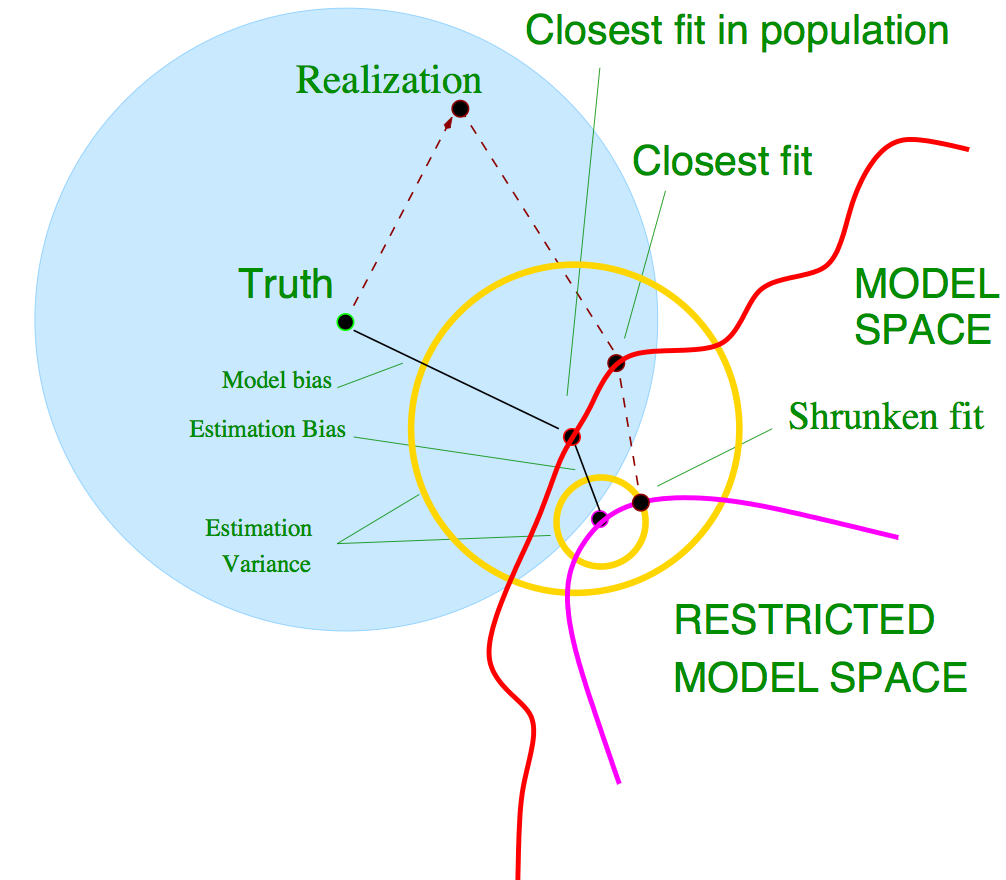
\includegraphics[width=\linewidth]{images/bias-variance.png}
\end{colfig}

Bias-variance come directly out of the test error:
 \begin{align*}
 \overline{teErr}
 &= E[(\text{observation} - \text{prediction})^2] = E[(y - \hat{y})^2] \\
 &= E[(y - y_{true} + y_{true} - \hat{y})^2] \\
 &=\underbrace{E[(y - y_{true})^2]}_{\text{var of measurement}} + E[(y_{true} - \hat{y})^2] \\
 &=\sigma^2 + E[(y_{true} - E[\hat{y}] + E[\hat{y}] - \hat{y})^2] \\
 &=\sigma^2 + \underbrace{E[(y_{true} - E[\hat{y}])^2]}_{\text{pred bias}^2} +\underbrace{E[(E[\hat{y}] - \hat{y})^2]}_{\text{pred variance}}
\end{align*}

\begin{tabular}{ l || c | c }
                          & bias & variance \\
  \hline
  regularization          & +    & - \\
  reduce model complexity & +    & - \\
  more data               & -    & \\
  \hline
\end{tabular}

\subsection{Consistency}
An estimator is said to be consistent, if it eventually recovers the true parameters that generated the data as the sample size goes to infinity. Of course, this only makes sense if the data actually comes from the specified model, which is not usually the case. Nevertheless, it can be a useful theoretical property.

\subsection{Convexity}
f is called convex f: $\forall x_1, x_2 \in X, \forall t \in [0, 1]: \qquad f(tx_1+(1-t)x_2)\leq t f(x_1)+(1-t)f(x_2).$

\subsection{Efficiency}
An estimator is called efficient if it achives the Cramer-Rao lower bound:
$\Var{(\beta)} \geq 1/I(\beta)$, where I is the fisher information.

\subsection{Curse of dimensionality}
The main reason behind the curse is that, with the dimensionality increase, every data point becomes arbitrarily far
from every other data point and therefore the choice of nearest neighbor becomes random.
In high dimension, data only covers a tiny fraction of the input space, making generalization extremely difficult.
Or in other words, the volume of the space increases so fast that the available data become sparse.

\subsection{Primal vs. Dual}
Instead of working in the column space of our data, we can work in the row space:
$$\bf{\hat{y} = X \beta = X X^T \alpha = K \alpha}$$
where $\bf{\beta} \in \mathbb{R}^D$ and $\bf{\alpha} \in \mathbb{R}^N$
and (like magic) $\bf{K}$ shows up, the Kernel Matrix.

Representer Theorem: For any $\bf{\beta}$ minimizing
$$\min_\beta \sum_{n=1}^N \mathcal{L}(y_n, \bf{x}_n^T \bf{\beta}) + \sum_{d=1}^D \lambda \beta_d^2$$
there exists an $\bf{\alpha}$ such that $\bf{\beta = X^T \alpha}$.

When we have an explicit vector formulation of $\beta$, we can use the matrix inversion lemma to get it. E.g. for ridge regression:
$$\beta = (X^T X  + \lambda I_D)^{-1} X^T y = X^T \underbrace{(X X^T + \lambda I_N)^{-1} y}_{\alpha}$$

\todo[inline]{k-fold cross-validation, definition of Test-Error, Train-Error}

\todo[inline]{TODO: statistical/computational tradeoff}

\todo[inline]{Definitions of: Optimality, Identifiability}

% ---------- Footer
\hrule
\tiny
Rendered \today. Written by Dennis Meier and Merlin Nimier-David. Most material was taken from the lecture notes of \href{http://people.epfl.ch/228491}{Prof. Emtiaz Khan}.
\copyright Dennis Meier. This work is licensed under the Creative Commons Attribution-ShareAlike 3.0 Unported License.
To view a copy of this license, visit \href{http://creativecommons.org/licenses/by-sa/3.0/}{http://creativecommons.org/licenses/by-sa/3.0/} or
send a letter to Creative Commons, 444 Castro Street, Suite 900, Mountain View, California, 94041, USA.

\includegraphics{images/by-sa.png}

\end{multicols*}
\end{document}
